\documentclass{article}
\usepackage{graphicx,fancyhdr,amsmath,amssymb,amsthm,subfig,url,hyperref,epigraph,lipsum,wrapfig}
\usepackage[margin=1in]{geometry}
\setlength\epigraphwidth{.8\textwidth}

% Bibliography
\usepackage[backend=biber, style=authortitle-comp, maxcitenames=1, refsection=section]{biblatex}
\addbibresource{report.bib}

%----------------------- Macros and Definitions --------------------------

\renewcommand{\theenumi}{\bf \Alph{enumi}}

\fancypagestyle{plain}{}
\pagestyle{fancy}
\fancyhf{}
\fancyhead[RO]{\sffamily\large University of Delhi}
\fancyhead[LO]{\sffamily\large MCS-204 Advanced Computer Networks}
\fancyfoot[RO]{\sffamily\thepage}
\renewcommand{\headrulewidth}{1pt}
\renewcommand{\footrulewidth}{1pt}

\graphicspath{{figures/}}

%-------------------------------- Title ----------------------------------

\title{Emerging Trends in Mobile Communications}
\author{
    Samyak Ahuja \\
    \texttt{Class ID: 29}
    \and
    Mayank Kharbanda \\
    \texttt{Class ID: 16}
}

%--------------------------------- Text ----------------------------------

\begin{document}
\maketitle

%--------------------------------- Title ----------------------------------
\section{C-RAN}

\epigraph{...}

\subsection{Introduction}
Global mobile data traffic is increasing at a substantial rate. It is 
estimated that it will grow seven fold from 2017 to 2022, with cell 
network advances and cut off in data price. To satisfy the consumer 
demands the network capacity is to be increased. It can be done by adding 
cell sites or by implementing the techniques like Multiple Input Multiple 
Output(MIMO). But increasing cell sited requires high capital and also 
results in increase in interference.\textcite{hass11}

\subsection{Architecture}

\subsubsection{Traditional Macro Base}
In the traditional architecture, radio and baseband processing
is done inside a base station. The antenna
module is generally located near the radio module, coaxial cables
are used to connect them, signal loss associated with them is high. 
This architecture was popular during 1G and 2G mobile networks.


\subsubsection{Base station with RRH}
In the Remote Radio Head (RRH) architecture, 
the base station has two components namely, a radio unit and a
signal processing unit. The radio unit
is called a RRH or Remote Radio Unit (RRU). The signal
processing part is called a BBU or Data Unit (DU). 
This architecture was introduced during 3G networks and right now the 
majority of base stations use it.\\
The distance between a RRH and a BBU can be extended up
to 40 km, where the limitation is coming from processing and
propagation delay. In this architecture, the BBU equipment can be
placed in a more convenient place, enabling
cost savings on site rental and maintenance compared to
the traditional RAN architecture. RRHs can be placed up on poles, 
leveraging efficient cooling and saving on airconditioning in BBU housing. 
One BBU can serve many RRHs. RRHs can be connected to each other in a
daisy chained architecture. Common Public Radio Interface (CPRI) is the 
radio interface protocol widely used for IQ data transmission between RRHs 
and BBUs.

\begin{figure}[!h]
  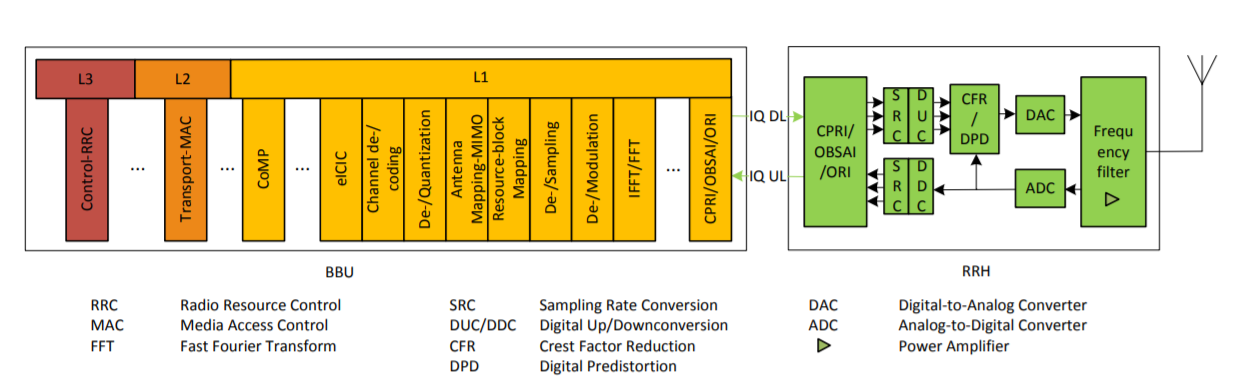
\includegraphics[width=\linewidth]{res/RRH_BBU_CRAN.PNG}
    \caption{Li-Fi}
  \label{fig:tech-illustration-li-fi}
\end{figure}

\begin{wrapfigure}{l}{0.5\textwidth}
  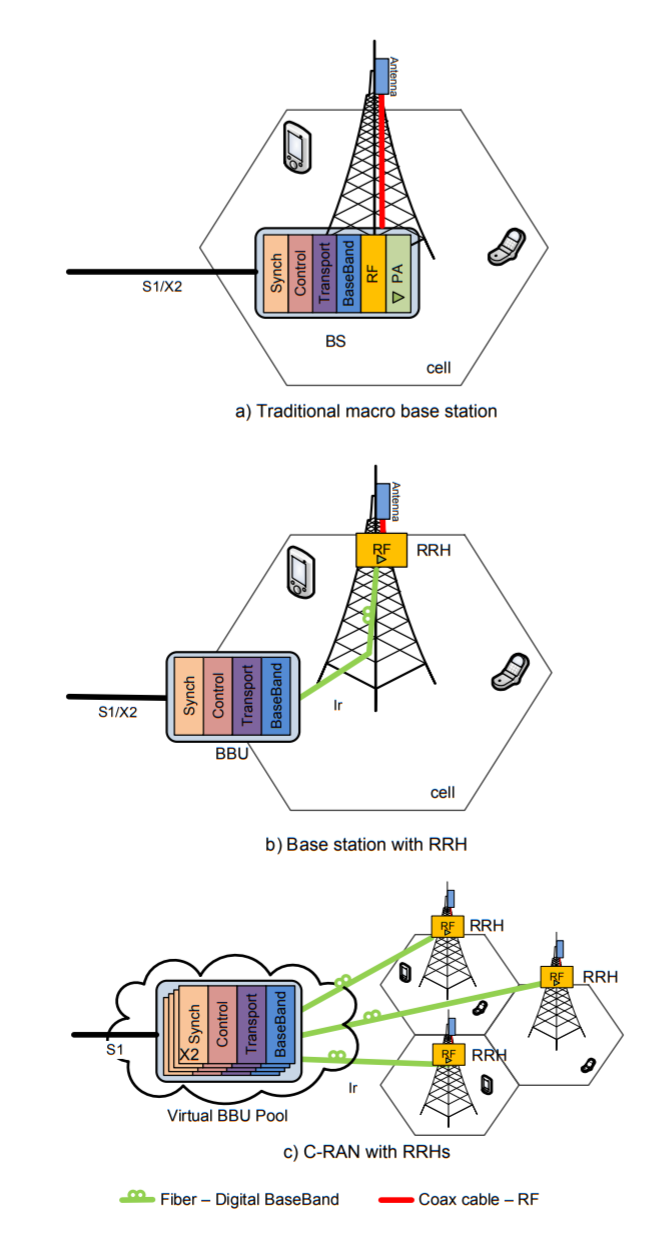
\includegraphics[scale=0.5]{res/compare_arc_CRAN.PNG}
    \caption{Li-Fi}
  \label{fig:tech-illustration-li-fi}
\end{wrapfigure}

\subsubsection{Centralized base station architecture, C-RAN} 
In C-RAN, in order to optimize BBU utilization between
heavily and lightly loaded base stations, the BBUs are 
centralized into one entity that is called a BBU Pool.
A BBU Pool acts as a virtualized cluster to perform baseband processing.
The concept of C-RAN was first introduced by IBM
under the name Wireless Network Cloud (WNC) and builds
on the concept of Distributed Wireless Communication System.
Since then various companies exploited the architecture and 
proposed improvements.\\

Figure 5 shows an example of a C-RAN mobile LTE
network. The fronthaul part of the network spans from the
RRHs sites to the BBU Pool. The backhaul connects the BBU
Pool with the mobile core network. At a remote site, RRHs are
co-located with the antennas. RRHs are connected to the high
performance processors in the BBU Pool through low latency,
high bandwidth optical transport links. Digital baseband, i.e.,
IQ samples, are sent between a RRH and a BBU.


\begin{wrapfigure}{r}{0.5\textwidth}
  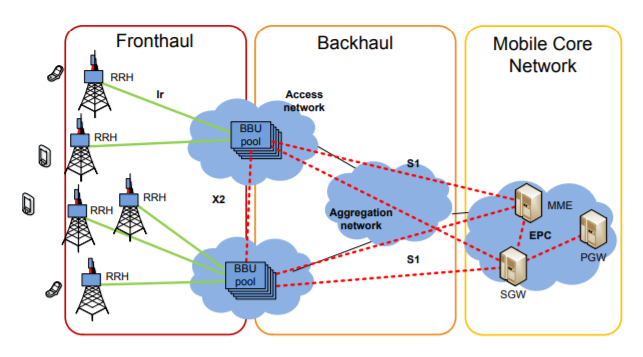
\includegraphics[scale=0.7]{res/LTE_CRAN.PNG}
    \caption{Li-Fi}
  \label{fig:tech-illustration-li-fi}
\end{wrapfigure}

\begin{figure}
  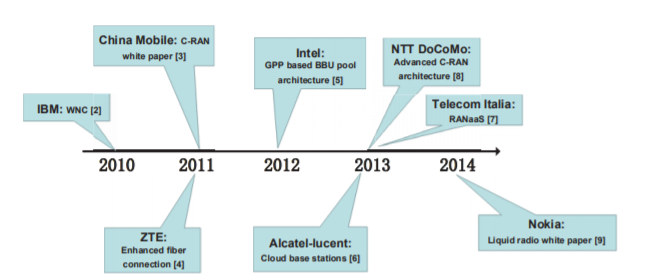
\includegraphics{res/arc_trend_CRAN.PNG}
    \caption{Li-Fi}
  \label{fig:tech-illustration-li-fi}
\end{figure}


\subsection{Advantages}

\begin{description}
    
    \item [Energy Efficient and Cost-saving] With centralized processing, 
    the number of BS 
    sites can be reduced. Thus the air conditioning and other site support 
    equipment's power consumption can be largely reduced. As the BBU pool 
    is a shared resource among a large number of virtual BS, it means a 
    much higher utilization rate of processing resources and lower power 
    consumption can be achieved.
    
    \item [Capacity Improvement] In C-RAN, virtual BS's can work together 
    in a large physical BBU pool and they can easily share the signaling, 
    traffic data and channel state information (CSI). 
    
    \item [Adaptability to Non-uniform Traffic] C-RAN is also suitable for 
    non-uniformly distributed traffic due to the load-balancing
    capability in the distributed BBU pool.
    
\end{description}




\printbibliography[heading=subbibliography]

\end{document}